\section{数值求积}
\label{sec:ru-numerical-quadrature}

原函数不便求出，或者被积函数只能在有限个点上计算时，需要用有限和近似积分。黎曼和本身就是一种近似，但取样点和权重可以选得更好。
本节先确定加权积分这一对象，再分别构造矩形、梯形与Simpson公式，比较它们所需的光滑条件与误差。

\subsection{加权积分}
\label{sec:ru-weighted-integrals}

许多累计量带有权重：密度不均匀的细杆，总质量是密度乘以长度的累计；不同位置重要性不同的误差，总误差也要按位置加权。
设$w,f$在有限区间$[a,b]$上连续，称$\int_a^bw(x)f(x)\,\mathrm dx$为$f$关于权函数$w$的加权积分，$w(x)$描述位置$x$的权重。$w\equiv1$时回到普通积分。
若$w\geq0$且总权重$\int_a^bw>0$，则
\[
 \frac{\int_a^bw(x)f(x)\,\mathrm dx}{\int_a^bw(x)\,\mathrm dx}
\]
称为$f$的加权平均。由$\min f\leq f\leq\max f$乘以$w\geq0$再积分，它介于$f$的最小值与最大值之间，正如有限个数的加权平均介于最小数与最大数之间。

数值求积把积分近似为有限个函数值的加权和
\[
 \int_a^bf(x)\,\mathrm dx\approx\sum_{i=0}^nc_if(x_i),
\]
其中$x_i$称为节点，$c_i$称为求积系数。求积系数是有限个数，权函数$w$是区间上的函数，两者不要混淆；对加权积分求积时，$w$的影响会体现在系数中。
举一个连续加权平均的例子：在$[0,1]$上取$w(x)=2x$，总权重为$1$，$f(x)=x^2$的普通平均为$\int_0^1x^2\,\mathrm dx=1/3$，加权平均为$\int_0^12x\cdot x^2\,\mathrm dx=1/2$，权重偏向右端，平均值随之增大。
概率中的密度与期望正是这种计算，见\BookChapterRef{chap:random-variables}{卷2《数学准备：概率、因果与决策》的“随机变量与概率基础”章}。

下面的求积公式都把$[a,b]$等分为$n$段，步长$h=(b-a)/n$，节点$x_k=a+kh$，并用同一个算例$\int_0^1e^x\,\mathrm dx=e-1\approx1.718282$核对，取$n=4$。

\subsection{矩形求积}
\label{sec:ru-rectangle-rule}

最简单的做法是在每段上把$f$近似为常数，即用一个矩形代替这一段。取左端点、右端点或中点的函数值作为高，分别得到复合左矩形、右矩形与中点公式，例如
\[
 L_n=h\sum_{k=0}^{n-1}f(x_k),\qquad M_n=h\sum_{k=0}^{n-1}f\Bigl(x_k+\frac h2\Bigr).
\]
算例中$L_4=0.25\,(e^0+e^{0.25}+e^{0.5}+e^{0.75})\approx1.512437$，误差约$0.206$；$M_4=0.25\,(e^{0.125}+e^{0.375}+e^{0.625}+e^{0.875})\approx1.713815$，误差约$0.0045$。同样只用四个函数值，中点公式精确得多。

这些公式都是黎曼和，$f$连续时由一致连续性随$h\to0$收敛到积分。误差的阶取决于光滑条件。设$|f'|\leq M_1$，在第$k$段上$|f(x)-f(x_k)|\leq M_1(x-x_k)$，积分得局部误差不超过$M_1h^2/2$，$n$段相加得
\[
 \Bigl|L_n-\int_a^bf\Bigr|\leq\frac{M_1(b-a)}2h.
\]
中点公式多了一层抵消。设$|f''|\leq M_2$，在中点$m$处展开$f(x)=f(m)+f'(m)(x-m)+\frac12f''(\xi_x)(x-m)^2$，一次项关于中点对称，积分为零，剩下的不超过$\frac{M_2}2\int(x-m)^2=M_2h^3/24$，于是
\[
 \Bigl|M_n-\int_a^bf\Bigr|\leq\frac{M_2(b-a)}{24}h^2.
\]
端点公式的误差与$h$同阶，只需要一阶导数有界；中点公式的误差与$h^2$同阶，要求二阶导数有界。算例中两个上界分别为$e/8\approx0.34$与$e/384\approx0.0071$，都覆盖了实际误差。

\subsection{梯形求积}
\label{sec:ru-trapezoid-rule}

把每段上的$f$近似为连接两端函数值的直线，就得到梯形公式：第$k$段的积分近似为$\frac h2\bigl(f(x_k)+f(x_{k+1})\bigr)$。相加时内部节点被相邻两段共用，所以
\[
 T_n=h\Bigl[\frac12f(x_0)+f(x_1)+\cdots+f(x_{n-1})+\frac12f(x_n)\Bigr],
\]
端点系数为$h/2$，内部节点系数为$h$。算例中$T_4\approx1.727222$，误差约$0.0089$。

误差来自直线插值的偏差。设$p$是第$k$段上的直线插值，对段内固定的$x$，令$\phi(t)=f(t)-p(t)-K(t-x_k)(t-x_{k+1})$，选$K$使$\phi(x)=0$。$\phi$有$x_k,x,x_{k+1}$三个零点，两次用Rolle定理得某个$\xi$使$\phi''(\xi)=0$，即$K=f''(\xi)/2$。于是
\[
 |f(x)-p(x)|\leq\frac{M_2}2(x-x_k)(x_{k+1}-x),
\]
积分得局部误差不超过$\frac{M_2}2\cdot\frac{h^3}6=M_2h^3/12$，整体误差不超过$M_2(b-a)h^2/12$。
梯形公式与中点公式的误差都是$h^2$阶，所需条件相同，界的常数却是$1/12$对$1/24$；算例中梯形误差约为中点误差的两倍，且符号相反（梯形偏大、中点偏小），这正是凸函数的弦在图像之上、切线在图像之下。

\subsection{Simpson求积}
\label{sec:ru-simpson-rule}

用二次多项式代替直线，可以进一步提高精度。在长为$2h$的区间$[m-h,m+h]$上取端点与中点三个函数值$f_-,f_0,f_+$，过这三点的二次多项式$p(x)=A+B(x-m)+C(x-m)^2$满足$A=f_0$、$2Ch^2=f_-+f_+-2f_0$，积分得
\[
 \int_{m-h}^{m+h}p(x)\,\mathrm dx=2Ah+\frac23Ch^3=\frac h3\bigl(f_-+4f_0+f_+\bigr).
\]
中点的权重$4$来自二次项的积分。由对称性，奇次项的积分为零，所以这一公式对三次多项式也精确。把$[a,b]$分为偶数$n$段，每相邻两段组成一组，得到复合Simpson公式
\[
 S_n=\frac h3\bigl[f(x_0)+4f(x_1)+2f(x_2)+4f(x_3)+\cdots+2f(x_{n-2})+4f(x_{n-1})+f(x_n)\bigr],
\]
$n$必须是偶数，组与组之间的共用节点系数为$2h/3$。算例中$S_4\approx1.718319$，误差约$3.7\times10^{-5}$，同样只用了五个函数值。

若$f$的四阶导数连续且$|f^{(4)}|\leq M_4$，复合Simpson公式的误差满足
\[
 \Bigl|S_n-\int_a^bf\Bigr|\leq\frac{M_4(b-a)}{180}h^4,
\]
证明与梯形公式类似，用三点插值的误差估计，并利用对称性多抵消一阶\scite{math-suli2003numerical}。算例中上界为$e/(180\cdot256)\approx5.9\times10^{-5}$。
图~\ref{fig:ru-quadrature-rules}比较了三种公式：在相同的函数值数量下，Simpson公式的误差随$n$下降得最快，代价是需要更高阶的光滑性；被积函数只有低阶导数有界时，高阶公式的优势随之消失。
对反常积分，先按上一节的尾部估计截断到有限区间，再在有限区间上求积，总误差是两部分之和；被积函数在端点有奇点时，导数无界，上面的误差界都不能直接使用。

\begin{figure*}[!htbp]
 \centering
 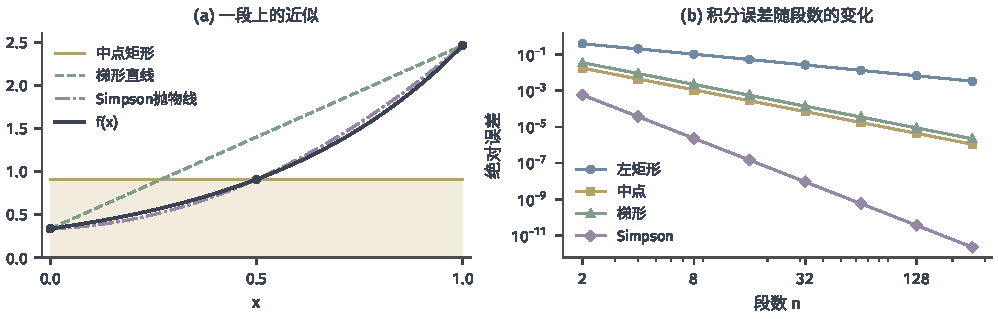
\includegraphics[width=169mm]{figures/01-mathematical-preliminaries-upper/02-real-numbers-and-univariate-functions/matplotlib/quadrature-rules/figure.pdf}
 \caption{三种求积公式的比较。(a)在一段$[0,1]$上近似$f(x)=e^{2x}/3$：中点公式用高为$f(1/2)$的矩形，梯形公式用连接两端的直线，Simpson公式用过两端与中点的抛物线，抛物线几乎与曲线重合。(b)$\int_0^1e^x\,\mathrm dx$的绝对误差随段数$n$变化，两轴均为对数刻度；左矩形、中点（与梯形）、Simpson的斜率分别约为$-1,-2,-4$，对应$h,h^2,h^4$阶误差。图为解析与双精度数值计算示例。}
 \label{fig:ru-quadrature-rules}
\end{figure*}
